%\begin{figure}[]\centering
%	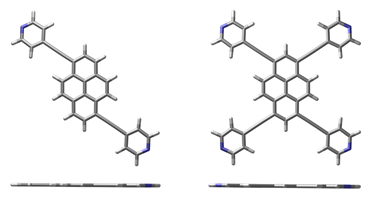
\includegraphics[width=0.7\textwidth]{./images/paper/pyrene/figure-S1}
%	\caption{Top and side views of optimized structures for trans-(left) and tetra-pyrene (right) at the B3LYP/6-31G(d,p) level of theory.}
%	\label{fig:pyene-S1}
%\end{figure}


%\begin{figure}[]\centering
%	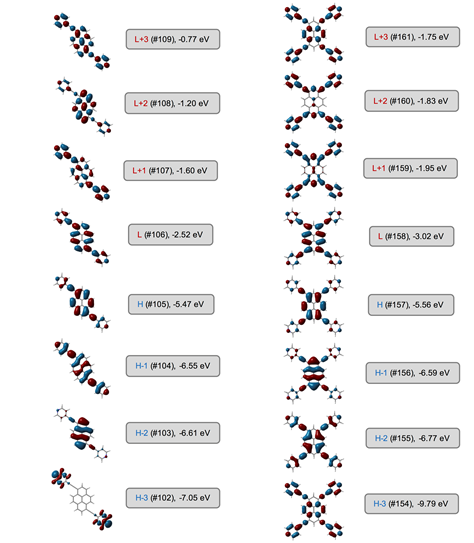
\includegraphics[width=0.7\textwidth]{./images/paper/pyrene/figure-S2}
%	\caption{Frontier molecular orbitals (isovalue contours ± 0.02 a.u.) for 1 (left) and 2 (right) from B3LYP/6-31G(d,p) calculations.}
%	\label{fig:pyene-S2}
%\end{figure}

%\begin{figure}[]\centering
%	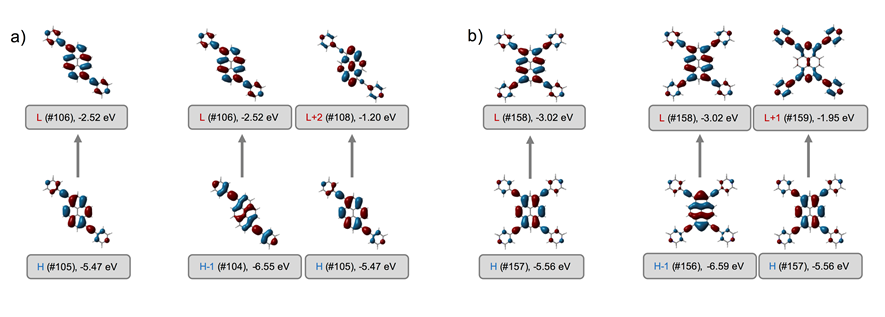
\includegraphics[width=0.7\textwidth]{./images/paper/pyrene/figure-S3}
%	\caption{Dominant orbital contributions to the first and second excitations in trans-pyrene (a) and in tetra-pyrene (b), obtained from TD-DFT calculations (CAM-B3LYP/6-31G**, toluene CPCM solvation).}
%	\label{fig:pyene-S3}
%\end{figure}

\begin{figure}[]\centering
	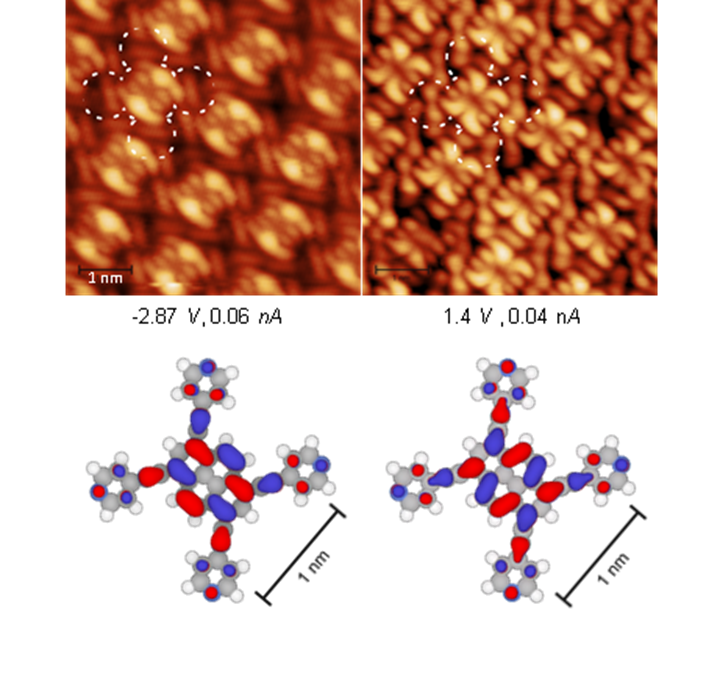
\includegraphics[width=0.7\textwidth]{./images/paper/pyrene/figure-S4}
	\caption{Calculated (EHT) HOMO (left) and LUMO (right) states of trans-pyrene. Assignment of HOMO and LUMO orbitals through symmetry observations in STM topography images that resolve the molecular orbitals. Compared to the HOMO, where between two legs only one side features a double lobe, the LUMO has double lobes in between every leg.}
	\label{fig:pyene-S4}
\end{figure}

\begin{figure}[]\centering
	\subfigure{
	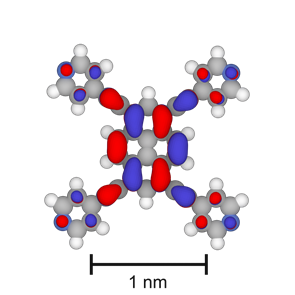
\includegraphics[width=0.35\textwidth]{./images/paper/pyrene/figure-S5a}
	\label{fig:pyrene-S5a}
	}
	\subfigure{
	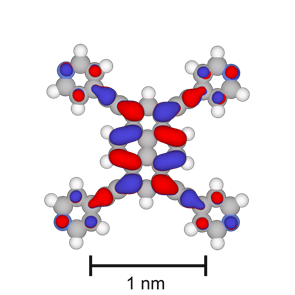
\includegraphics[width=0.35\textwidth]{./images/paper/pyrene/figure-S5b}
	\label{fig:pyrene-S5b}
	}
	\caption{a) EHT calculated HOMO and b) LUMO states of cis-pyrene.}
	\label{fig:pyene-S5}
\end{figure}

\autoref{fig:pyene-S6} shows the emergence of LUMO states for trans-pyrene. The STM topographies show the same region with subsequently increased bias voltage. Starting close to the fermi level in the molecules’ band gap the contrast is determined by the shape of the molecule (upper left). Increasing the bias voltage (for upper left to lower right) reveals two things. First the contrast pattern changes at energies close to the proposed LUMO \SIrange{1.4}{1.6}{\volt} and LUMO + 1 \SIrange{2.2}{2.4}{\volt} energies, while the contrast between \SI{1.8}{\volt} and \SI{2.1}{\volt} remains constant. Second this change in contrast is not homogeneous across the surface but originates from the pores´ center.

\begin{figure}[]\centering
	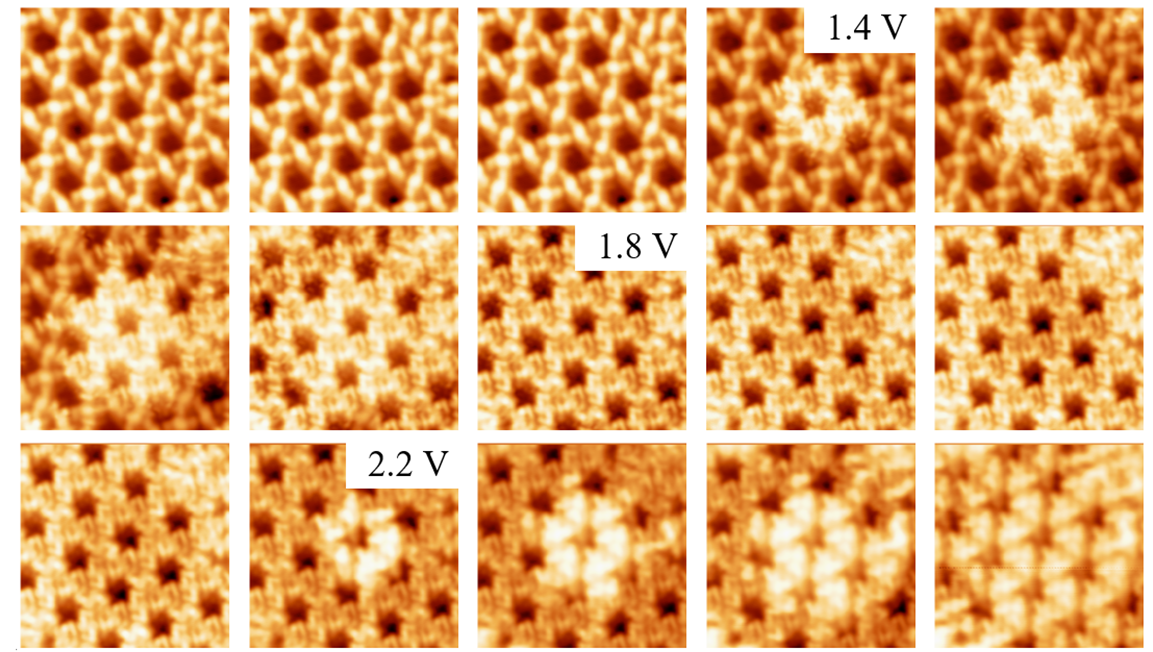
\includegraphics[width=0.7\textwidth]{./images/paper/pyrene/figure-S6}
	\caption{STM image series depicting LUMO/LUMO+1 states with positive bias voltages (\SIrange{1.1}{2.5}{\volt}). Starts @ \SI{1.1}{\volt} and increases in steps of \SI{0.1}{\volt} for upper left to lower right, Image size is \SI{11}{\nano \meter} $\times$ \SI{11}{\nano \meter}.}
	\label{fig:pyene-S6}
\end{figure}

\begin{figure}[]\centering
	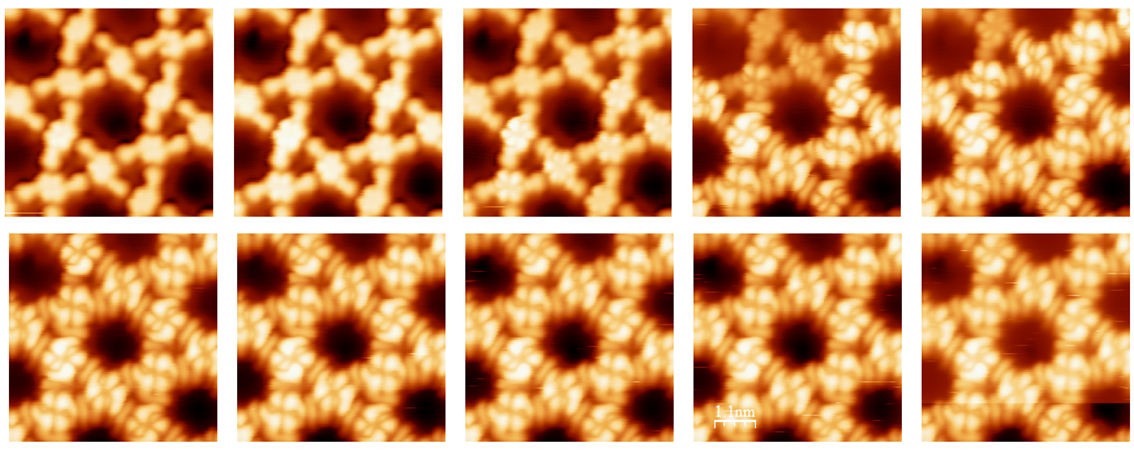
\includegraphics[width=0.7\textwidth]{./images/paper/pyrene/figure-S7}
	\caption{STM image series depicting HOMO-1 states with negative bias voltages \SIrange{-1.8}{-2.7}{\volt}. Starts @ \SI{-1.8}{\volt} and decreases in steps of \SI{0.1}{\volt} for upper left to lower right. Image size is \SI{5.5}{\nano \meter} $\times$ \SI{5.5}{\nano \meter}.
	}
	\label{fig:pyene-S7}
\end{figure}

\begin{figure}[]\centering
	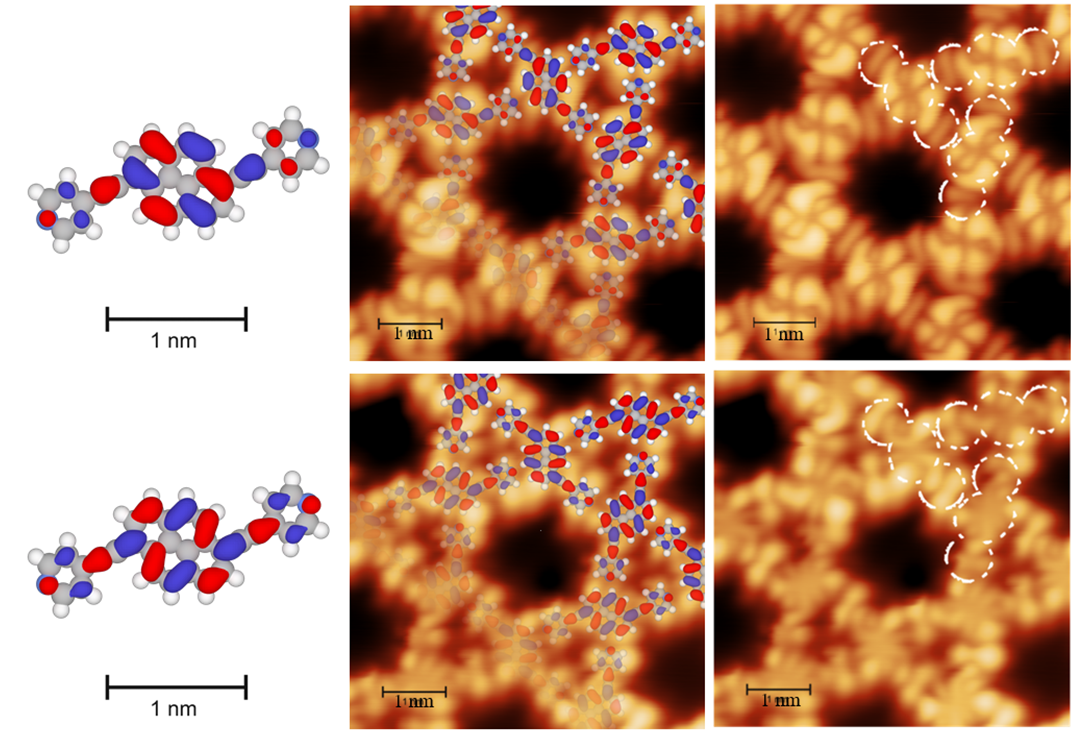
\includegraphics[width=0.7\textwidth]{./images/paper/pyrene/figure-S8}
	\caption{Calculated (EHT) HOMO (top) and LUMO (bottom) states (in red/blue) superimposed on a model of trans-pyrene. Imaging parameter: \SI{-2.4}{\volt} (HOMO) \& 2.1 V (LUMO). Recorded with \SI{0.2}{\nano \ampere}, Image width: \SI{5.5}{\nano \meter}.
	}
	\label{fig:pyene-S8}
\end{figure}

\begin{figure}[]\centering
	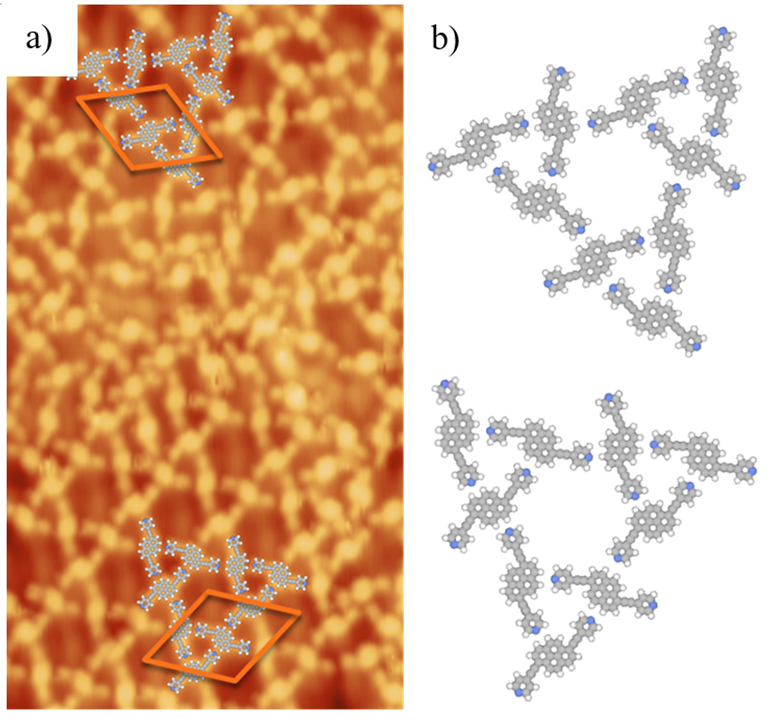
\includegraphics[width=0.7\textwidth]{./images/paper/pyrene/figure-S9}
	\caption{Homochiral mirror domains of a self-assembled sub-ML of trans-pyrene on h-BN/Cu(111). a) STM image with overlaid molecular models and unit cells (colored in orange). b) Enlarged view on the molecular assembly in a). Imaging parameters: \SI{14}{\nano \meter} $\times$ \SI{25}{\nano \meter}, \SI{1.0}{\volt}, \SI{0.1}{\nano \ampere}.
	}
	\label{fig:pyene-S9}
\end{figure}

Some preparations were done to show the functionality of the trans-pyrene pores as host system for other molecules. First cis-pyrene was dosed on the surface at R, afterwards annealed to 100°C, cooled to RT followed by dosing trans-pyrene molecules. Two different, coexisting motifs occur which are shown in Figure S10. First there is a dense packed phase (Figure S10a, c). This mixed preparation does show a uniform growth. Alternating rows of either trans-pyrene or pairs of cis-pyrene molecules assemble in islands. The resulting triclinic unit cell (\SI{1.94}{\nano \meter} $\times$ \SI{1.97}{\nano \meter} \SI{75}{\degree}) incorporates 3 molecules – one trans-pyrene and two cis-pyrenes. The second phase is dominated by the kagome motif already observed in the homo-molecular preparations but with their larger pores partially filled with cis-pyrene species (Figure S10b, d). The unit cell remains the very same, but contains an additional cis-pyrene molecule. Not all guests (cis-pyrene) molecules are oriented the same way, only discrete orientations are allowed (and three of six different ones can already be seen in Figure S10b). This means that although cis-pyrene molecules were evaporated first their assembly becomes unstable at temperatures of about \SI{100}{\celsius}. This allows them to participate in the nucleation process after the trans-pyrene molecules are dosed at RT. Their assembly is still in progress while cooling down from RT to \SI{7}{\Kelvin}. A fully occupied kagome cell bears 3 trans-pyrene molecules and a single cis-pyrene molecule.

\begin{figure}[]\centering	
	\subfigure[]{
	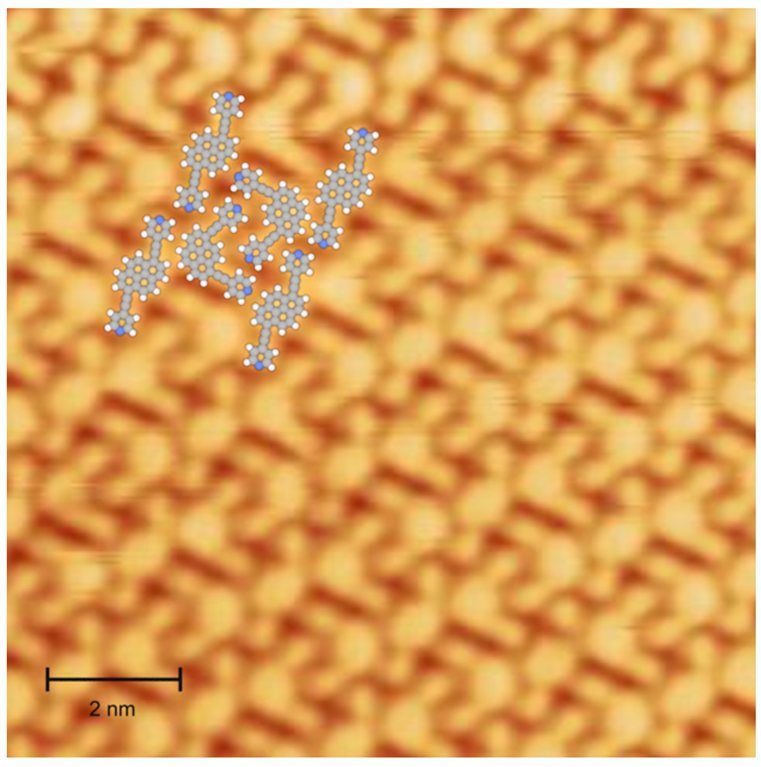
\includegraphics[width=0.35\textwidth]{./images/paper/pyrene/figure-S10a}
		\label{fig:pyrene-S10a}
	}
	\subfigure[]{
	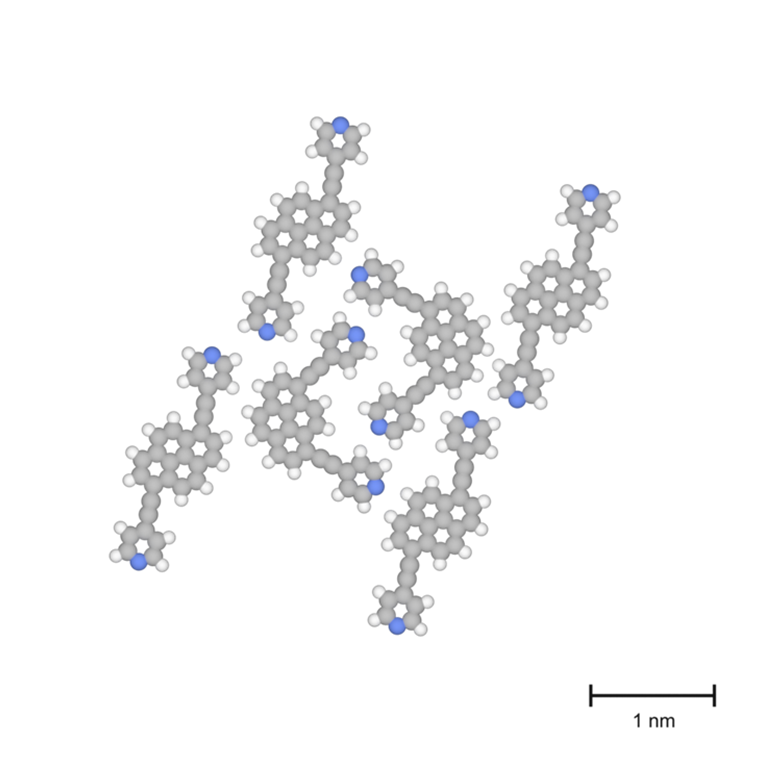
\includegraphics[width=0.35\textwidth]{./images/paper/pyrene/figure-S10b}
		\label{fig:pyrene-S10b}
	}
	\subfigure[]{
	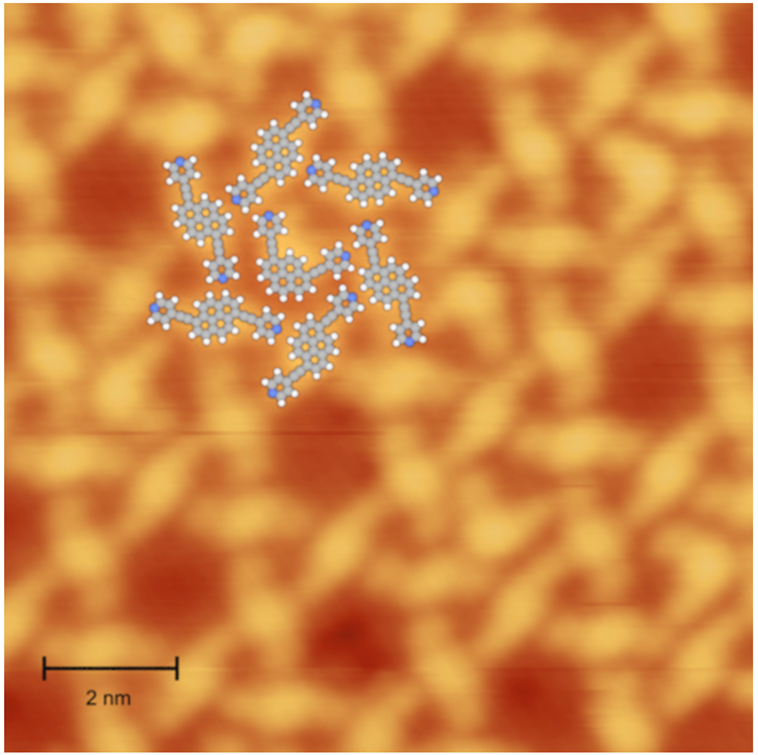
\includegraphics[width=0.35\textwidth]{./images/paper/pyrene/figure-S10c}
		\label{fig:pyrene-S10c}
	}
	\subfigure[]{
	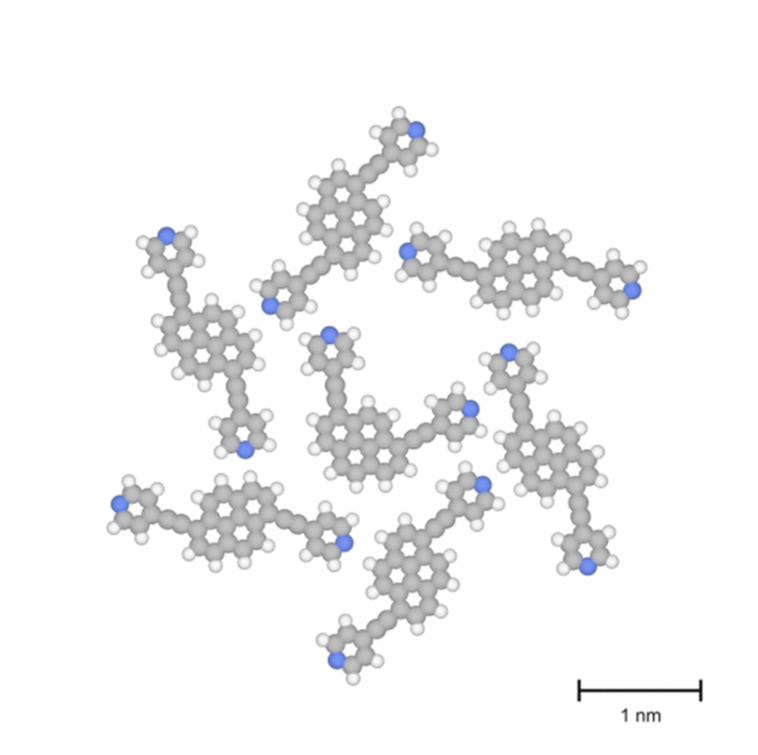
\includegraphics[width=0.35\textwidth]{./images/paper/pyrene/figure-S10d}
		\label{fig:pyrene-S10d}
	}	
	\caption{Cis-pyrene/trans-pyrene mixed preparation on \textit{h}-BN/Cu (111). STM image of a self-assembled sub-ML with overlaid molecular models (\subref{fig:pyrene-S10a}, \subref{fig:pyrene-S10c}). Enlarged views on the molecular unit cells (\subref{fig:pyrene-S10b}, \subref{fig:pyrene-S10d}). \subref{fig:pyrene-S10a}, \subref{fig:pyrene-S10b}) shows a dense packed mixed motif while \subref{fig:pyrene-S10c} and \subref{fig:pyrene-S10d} show cis-pyrene molecules (guest) in a trans-pyrene kagome (host) network. Imaging parameters: \SI{1.0}{\volt}, \SI{0.06}{\nano \ampere}.
		%, \SI{}{\nano \meter} $\times$ \SI{}{\nano \meter}.
	}
	\label{fig:pyene-S10}
\end{figure}

%\begin{figure}[]\centering
%	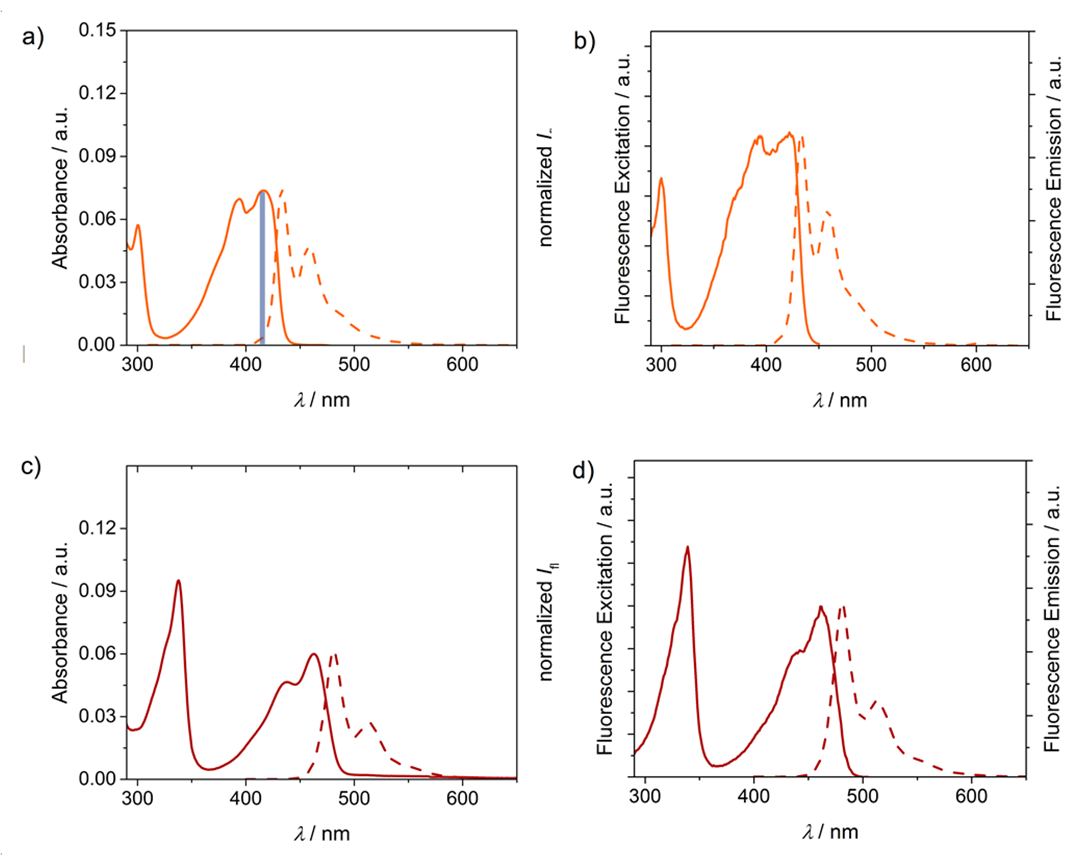
\includegraphics[width=0.7\textwidth]{./images/paper/pyrene/figure-S11}
%	\caption{Absorption and emission spectra for trans- and tetra-pyrene.
%	}
%	\label{fig:pyene-S11}
%\end{figure}

%\begin{figure}[]\centering
%	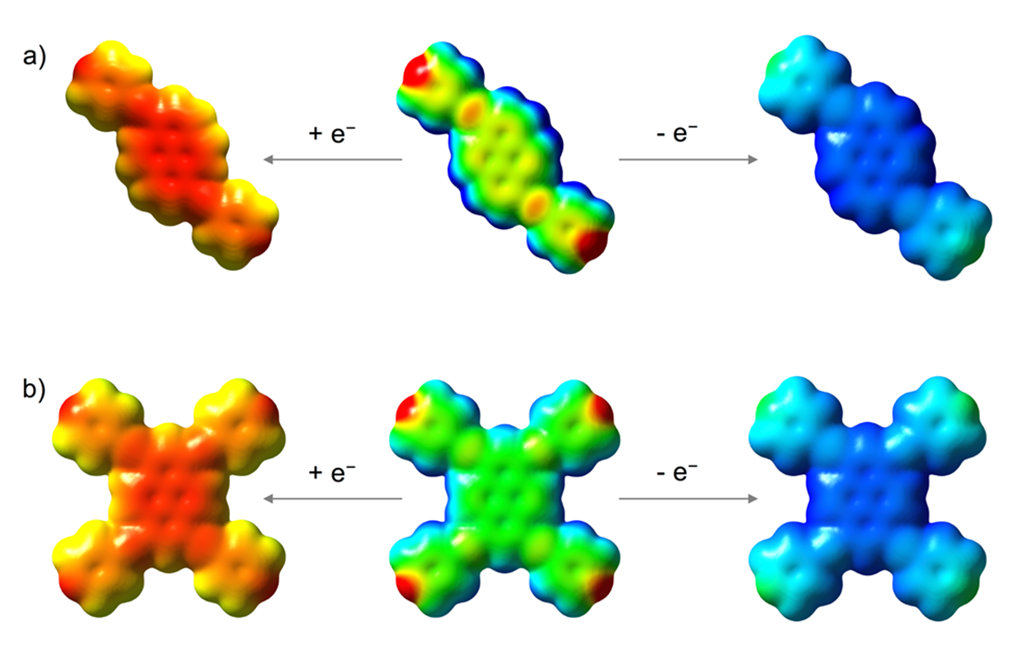
\includegraphics[width=0.7\textwidth]{./images/paper/pyrene/figure-S12}
%	\caption{Mapped Electrostatic Potential of trans-pyrene (top) and tetra-pyrene (bottom).
%	}
%	\label{fig:pyene-S12}
%\end{figure}

%\begin{figure}[]\centering
%	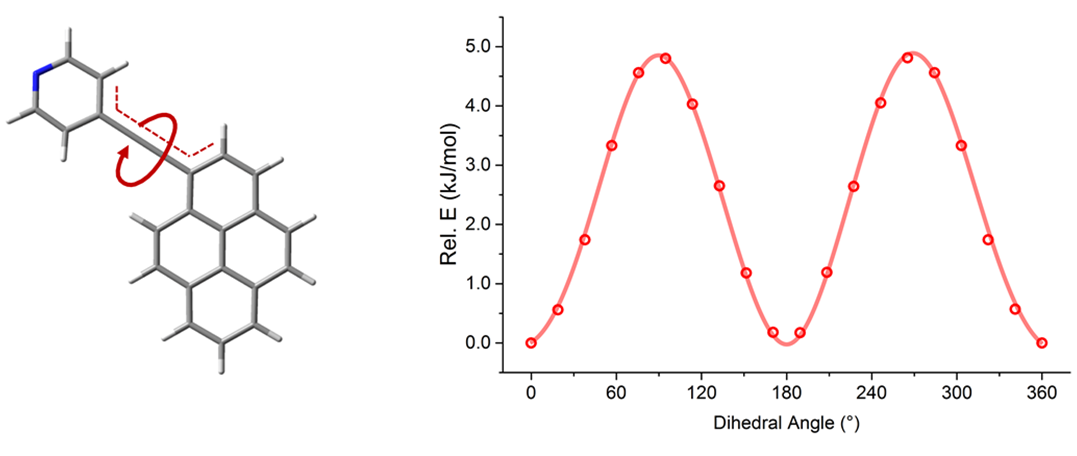
\includegraphics[width=0.7\textwidth]{./images/paper/pyrene/figure-S13}
%	\caption{Model pyridylethynyl pyrene compound used for calculating the energy profile for the rotation around the triple bond, at the B3LYP/6-31G(d,p) level of theory.
%	}
%	\label{fig:pyene-S13}
%\end{figure}
